\chapter{Integrationstests}

\section{Test 1 - Gleichm��iges Publizieren }
Dieser Test pr�ft, ob bei stetigem Publizieren die Frequenz korrekt bewertet wird und ob auf die Bewertung korrekt reagiert wird.

\begin{enumerate}
    \item Test-Launchfile starten:
    Mit \texttt{roslaunch arni\_core test\_1\_steady.launch} wird das Launchfile gestartet.\\
    Man sieht, dass dabei folgende Knoten gestartet werden:
    \begin{verbatim}
        countermeasure (arni_countermeasure/arni_countermeasure)
        ninja_turtle (arni_core/predefined_subscriber.py)
        node_manager (arni_nodeinterface/arni_nodeinterface)
        processing (arni_processing/arni_processing)
        steady_tree (arni_core/predefined_publisher.py)
    \end{verbatim}
    Debei besteht folgende Verbindung der Knoten (Debugging-Knoten zur �bersichtlichkeit ausgenommen):\\

\begin{figure}[htbp]
    \begin{minipage}[t]{16cm}
        \vspace{0pt}
        \centering
        
\includegraphics[scale=0.3]{./bilder/integrationstests/test_1_nodegraph.png}
        \caption{steady\_tree publiziert mit 100Hz auf /forest, ninja\_turtle abonniert forest.}
    \end{minipage}
    \hfill
\end{figure}  

    Die Frequenz von /forest wird unter 80Hz als LOW und �ber 120Hz als HIGH bewertet.
    Der Countermeasure-Knoten hat das Constraint alle 10 Sekunden \textit{frequency of forest is ok} auszugeben, falls die Frequenz mit OK bewertet wurde.

\newpage
    \item �ffnen der GUI:
    In die Konsole wird \texttt{rosrun rqt\_gui rqt\_gui} eingegeben und ausgef�hrt.\\
    \item �ffnen der Widgets:
    Ausw�hlen des Widgets \textit{Logging > Console},\\
    Debug Messages ausblenden\\

\begin{figure}[htbp]
    \begin{minipage}[t]{16cm}
        \vspace{0pt}
        \centering
        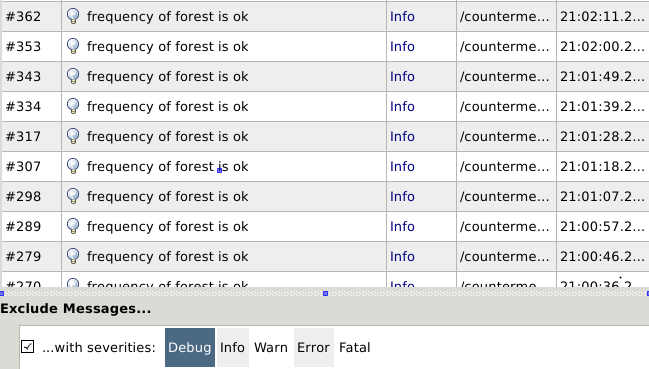
\includegraphics[scale=0.5]{./bilder/integrationstests/test_1_rqt_freq_ok.png}
        \caption{steady\_tree publiziert mit 100Hz auf forest. ninja\_turtle h�rt zu.}
    \end{minipage}
    \hfill
\end{figure}  


    Es ist zu sehen, dass die Nachricht des Countermeasure-Knotens alle 10 Sekunden publiziert wird.
\end{enumerate}


\newpage
\section{Test 2 - Zu niedrige Frequenz }
Dieser Test pr�ft das Verhalten beim Publizieren mit geringerer Frequenz als durch die Spezifikationen erwartet wird und ob auf die Bewertung korrekt reagiert wird.

\begin{enumerate}
    \item Test-Launchfile starten:
    Mit \texttt{roslaunch arni\_core test\_2\_steady\_low.launch} wird das Launchfile gestartet.\\
    Man sieht, dass dabei folgende Knoten gestartet werden:
    \begin{verbatim}
        countermeasure (arni_countermeasure/arni_countermeasure)
        leopard_seal (arni_core/predefined_subscriber.py)
        node_manager (arni_nodeinterface/arni_nodeinterface)
        processing (arni_processing/arni_processing)
        breathing_penguin (arni_core/predefined_publisher.py)
    \end{verbatim}
    Debei besteht folgende Verbindung der Knoten (Debugging-Knoten zur �bersichtlichkeit ausgenommen):\\

\begin{figure}[htbp]
    \begin{minipage}[t]{16cm}
        \vspace{0pt}
        \centering
        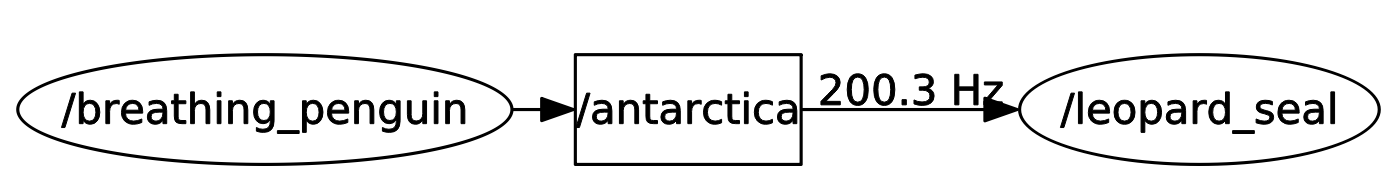
\includegraphics[scale=0.3]{./bilder/integrationstests/test_2_nodegraph.png}
        \caption{breathing\_penguin publiziert mit 200Hz auf /antarctica, leopard\_seal abonniert antarctica.}
    \end{minipage}
    \hfill
\end{figure}  

    Die Frequenz von /antarctica wird unter 400Hz als LOW und �ber 600Hz als HIGH bewertet.
    Der Countermeasure-Knoten hat das Constraint alle 5 Sekunden \textit{frequency of antarctica is too low} auszugeben, falls die Frequenz mit LOW bewertet wurde.

\newpage
    \item �ffnen der GUI:
    In die Konsole wird \texttt{rosrun rqt\_gui rqt\_gui} eingegeben und ausgef�hrt.\\
    \item �ffnen der Widgets:
    Ausw�hlen des Widgets \textit{Logging > Console},\\
    Debug Messages ausblenden\\

\begin{figure}[htbp]
    \begin{minipage}[t]{16cm}
        \vspace{0pt}
        \centering
        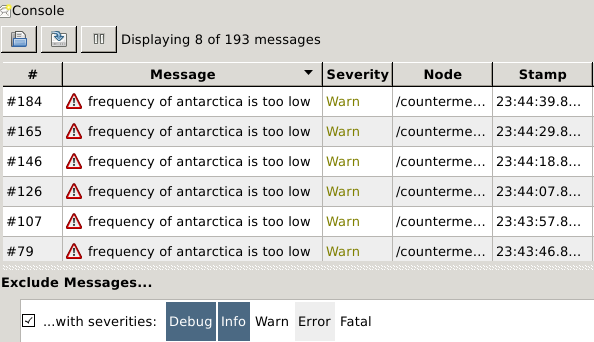
\includegraphics[scale=0.5]{./bilder/integrationstests/test_2_log.png}
        \caption{breathing\_penguin publiziert mit 200Hz auf /antarctica. leopard\_seal h�rt zu.}
    \end{minipage}
    \hfill
\end{figure}  


    Es ist zu sehen, dass die Nachricht des Countermeasure-Knotens alle 5 Sekunden publiziert wird.
\end{enumerate}


\newpage
\section{Test 3 - Variierende Frequenz }
Dieser Test pr�ft das Verhalten beim Publizieren mit variierender Frequenz in einer Sinuskurve, wobei hohe Werte als zu hoch und niedrige Werte als zu niedrig bewertet werden.

\begin{enumerate}
    \item Test-Launchfile starten:
    Mit \texttt{roslaunch arni\_core test\_3\_fluctuation.launch} wird das Launchfile gestartet.\\
    Man sieht, dass dabei folgende Knoten gestartet werden:
    \begin{verbatim}
        countermeasure (arni_countermeasure/arni_countermeasure)
        sailing_boat (arni_core/predefined_subscriber.py)
        node_manager (arni_nodeinterface/arni_nodeinterface)
        processing (arni_processing/arni_processing)
        fluctuation_tide (arni_core/predefined_publisher.py)
    \end{verbatim}
    Debei besteht folgende Verbindung der Knoten (Debugging-Knoten zur �bersichtlichkeit ausgenommen):\\

\begin{figure}[htbp]
    \begin{minipage}[t]{16cm}
        \vspace{0pt}
        \centering
        
\includegraphics[scale=0.3]{./bilder/integrationstests/test_3_nodegraph.png} % TODO: neues bild
        \caption{fluctuation\_tide publiziert mit einer Frequenz zwischen 10 und 190 auf /ocean, sailing\_boat abonniert ocean.}
    \end{minipage}
    \hfill
\end{figure}  

    Die Frequenz von /ocean wird unter 70Hz als LOW und �ber 130Hz als HIGH bewertet.
    Unterschreitet die aufgezeichnete Frequenz die Grenze, wird \textit{frequency of ocean is too low} auszugeben, \textit{frequency of ocean is too high}, wenn die Frequenz 130Hz �berschreitet und \textit{frequency of ocean is ok} sonst.

\newpage
    \item �ffnen der GUI:
    In die Konsole wird \texttt{rosrun rqt\_gui rqt\_gui} eingegeben und ausgef�hrt.\\
    \item �ffnen der Widgets:
    Ausw�hlen des Widgets \textit{Logging > Console},\\
    Debug Messages ausblenden\\

\begin{figure}[htbp]
    \begin{minipage}[t]{16cm}
        \vspace{0pt}
        \centering
        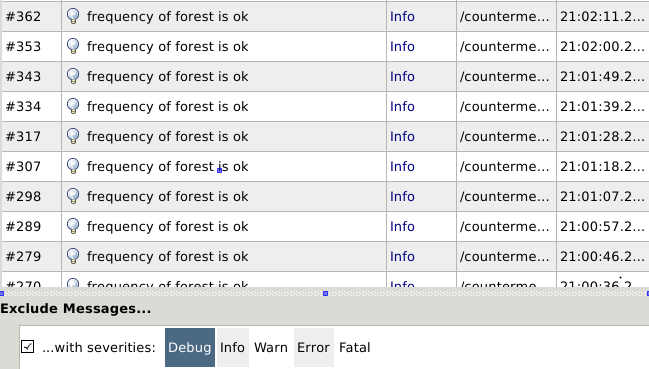
\includegraphics[scale=0.5]{./bilder/integrationstests/test_1_rqt_freq_ok.png} % TODO: neues bild
        \caption{fluctuation\_tide publiziert mit 10 - 190Hz auf /ocean. sailing\_boat h�rt zu.}
    \end{minipage}
    \hfill
\end{figure}

    \item �ffnen der Arni-Widgets:
    Ausw�hlen des Widgets \textit{Introspection > Arni-Detail}, bei Filter wird \texttt{ocean} eingegeben und die Eingabe best�tigt. Im Baum wird \texttt{t!/ocean} ausgew�hlt.
    Im Fenster auf der rechten Seite wird der Reiter \textit{Graphs} ausgew�hlt. Darunter wird Range auf \texttt{60 Seconds} und Selected auf \texttt{delivered_msgs, frequency} gestellt.
    Man sieht eine stufige Sinuskurve, die sich langsam ausbreitet.


    Es ist zu sehen, dass sich \textit{[...] is ok}, \textit{[...] is too high}, \textit{[...] is ok}, \textit{[...] is too low}, etc. abwechseln.
\end{enumerate}


\newpage
\section{Test 4 - Neustarten eines Knotens}
Der Knoten in diesem Test sendet nach 100 Sekunden mit stark reduzierter Frequenz und wird daraufhin vom Countermeasure Knoten neugestartet.

\begin{enumerate}
	\item Test-Launchfile starten:
	Mit \texttt{roslaunch arni\_core test\_4\_restarting.launch} wird das Launchfile gestartet.\\
	Man sieht, dass dabei folgende Knoten gestartet werden:
	\begin{verbatim}
	    countermeasure (arni_countermeasure/arni_countermeasure)
	    sturbacks (arni_core/predefined_subscriber.py)
	    node_manager (arni_nodeinterface/arni_nodeinterface)
	    processing (arni_processing/arni_processing)
	    jumping_tower (arni_core/predefined_publisher.py)
	\end{verbatim}
	Debei besteht folgende Verbindung der Knoten (Debugging-Knoten zur �bersichtlichkeit ausgenommen):\\

\begin{figure}[htbp]
    \begin{minipage}[t]{16cm}
        \vspace{0pt}
        \centering
        
\includegraphics[scale=0.3]{./bilder/integrationstests/test_3_nodegraph.png} % TODO: neues bild
        \caption{jumping\_tower publiziert f�r 100 Sekunden mit 100Hz auf /street, sturbacks abonniert street.}
    \end{minipage}
    \hfill
\end{figure}  

    Die Frequenz von /ocean wird unter 80Hz als LOW bewertet.
    Unterschreitet die aufgezeichnete Frequenz die Grenze, wird \textit{frequency of street is too low - trying to restart} auszugeben und der Knoten wird neugestartet.\\
    Bis dahin und danach wird \textit{frequency of street is ok} geloggt.

    % TODO: bis hierhin und nicht weiter :D

\newpage
	\item �ffnen der GUI:
	In die Konsole wird \texttt{rosrun rqt\_gui rqt\_gui} eingegeben und ausgef�hrt.\\
	\item �ffnen der Widgets:
	Ausw�hlen des Widgets \textit{Logging > Console},\\
    Debug Messages ausblenden\\

\begin{figure}[htbp]
    \begin{minipage}[t]{16cm}
        \vspace{0pt}
        \centering
        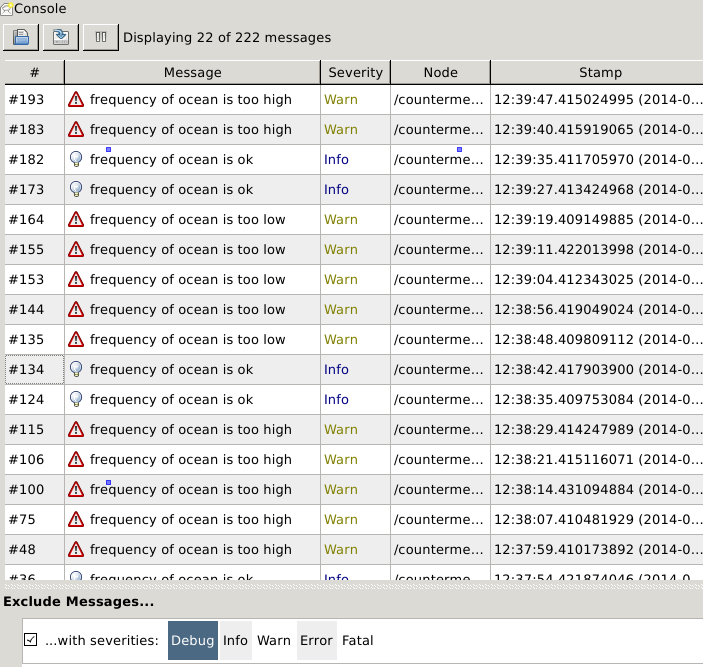
\includegraphics[scale=0.5]{./bilder/integrationstests/test_3_log.png}
        \caption{fluctuation\_tide publiziert mit 10 - 190Hz auf /ocean. sailing\_boat h�rt zu.}
    \end{minipage}
    \hfill
\end{figure}  


    Es ist zu sehen, dass sich \textit{[...] is ok}, \textit{[...] is too high}, \textit{[...] is ok}, \textit{[...] is too low}, etc. abwechseln.
\end{enumerate}
